\chapter{Datos y metodología}
\label{cap:datos}

\section{Fuente, alcance y estado del diseño}

ENASEM es un estudio longitudinal nacional que examina salud y envejecimiento
desde una perspectiva socioeconómica. El perfil de cohorte de
\citet{wong2017} describe la muestra basal de 2001, el seguimiento y la
incorporación de una cohorte adicional en 2012. Esa publicación antecede a
varias rondas incluidas aquí; la cobertura de seis rondas se documenta en la
versión de ENASEMsimple utilizada, no se atribuye retrospectivamente al
artículo de cohorte. El diccionario de 2025 identifica las rondas nominales
2001, 2003, 2012, 2015, 2018 y 2021 \citep{enasem2025simple}.

La base local \variable{simpleMHAS.dta} contiene una selección de variables,
en lugar de la totalidad de los instrumentos originales. El presente capítulo
se apoya en la auditoría CP1, los informes de revisión y las tablas agregadas
reproducibles del proyecto. Se diferencian dos planos: los procedimientos y
resultados descriptivos ya ejecutados, y las decisiones del diseño predictivo
que todavía necesitan aprobación. No se han construido etiquetas ni estimado
modelos. El EDA independiente por bloques se inició después de la revisión
del inventario, por autorización explícita de la autora; se documenta en
la sección~\ref{sec:eda-independiente-metodo}.

La referencia descriptiva conserva toda la población registrada. No se aplica
un filtro inicial de edad, modalidad o continuidad. Esta decisión de alcance
permite examinar posteriormente qué información elimina cada alternativa de
muestra, sin convertir la población de 60 años o más en una restricción para
toda la investigación. El universo registrado tampoco equivale a todos los
intentos de contacto ni a la totalidad de la población mexicana.

\section{Unidad de observación e integridad del panel}

La unidad de observación del archivo es la persona-ronda: una entrevista
completada por la persona o en su nombre. La unidad de enlace longitudinal es
la persona identificada internamente por la combinación de \variable{cunicah}
y \variable{np}. Al añadir \variable{ronda} se obtiene la clave de observación.
La auditoría verificó integridad de claves y unicidad antes de enlazar rondas;
no detectó claves faltantes ni duplicados persona-ronda. Por tanto, el número
de registros coincide con el número de personas dentro de una ronda, aunque
no en el conjunto del periodo.

El archivo conserva \cpTotalRegistros{} registros, \cpTotalPersonas{} personas
únicas y \cpTotalVariables{} columnas originales. El cociente entre registros
y personas no debe interpretarse como un periodo de seguimiento uniforme:
cada historia contiene de una a seis observaciones y los intervalos de las
rondas son desiguales. Los identificadores se conservan en archivos privados para
validación y enlace; el manuscrito publica exclusivamente conteos agregados.

Formalmente, se define la presencia como
\begin{equation}
 R_{ir}=\mathbf{1}\{\text{existe un registro de la persona }i
                         \text{ en la ronda }r\},\qquad
 K_i=\sum_{r=1}^{6}R_{ir}.
 \label{eq:presencia}
\end{equation}
El indicador $R_{ir}$ incluye entrevistas directas, por sustituto y sobre
fallecidos. Describe existencia de un registro, no una certificación de que
la persona estaba viva o respondió directamente en ese momento. De aquí se
obtiene la reconciliación $\sum_i K_i=\cpTotalRegistros{}$, mientras que el
número de historias individuales es \cpTotalPersonas{}.

% Generado: no editar cifras manualmente.
\begin{table}[!htbp]
\centering
\caption{Población registrada en las seis rondas}\label{tab:cp1-rondas}
\small\setlength{\tabcolsep}{4pt}
\renewcommand{\arraystretch}{1.15}
\begin{tabular}{lrrrrr}
\toprule
\textbf{Año} & \textbf{Registros} & \textbf{Personas} & \textbf{Menores de 60} & \textbf{60+} & \textbf{Edad faltante} \\
\midrule
2001 & 15\,186 & 15\,186 & 7\,770 & 7\,416 & 0 \\
2003 & 14\,250 & 14\,250 & 6\,002 & 7\,691 & 557 \\
2012 & 18\,465 & 18\,465 & 5\,815 & 9\,886 & 2\,764 \\
2015 & 15\,988 & 15\,988 & 4\,359 & 10\,416 & 1\,213 \\
2018 & 18\,249 & 18\,249 & 6\,981 & 10\,113 & 1\,155 \\
2021 & 17\,538 & 17\,538 & 5\,247 & 10\,482 & 1\,809 \\
\bottomrule
\end{tabular}
\par\medskip
\parbox{\linewidth}{\footnotesize Fuente: elaboración propia con agregados de CP1, ENASEMsimple v2 (2001--2021). Frecuencias sin ponderación. N de personas dentro de cada ronda; no se suman para obtener personas únicas del periodo. Todas las edades y modalidades.}
\end{table}


\section{Rondas nominales y cronología efectiva}

La tabla~\ref{tab:cp1-rondas} resume las seis rondas y distingue edad válida
menor de 60, edad válida de 60 o más y edad faltante. La presencia de menores
de 50 es compatible con el reclutamiento de cónyuges sin restricción de edad
descrito por el proveedor \citep[p.~2]{enasem2025simple}; no se considera un
error por el solo hecho de estar por debajo de ese umbral.

La ronda nominal, almacenada en \variable{ronda}, se mantiene separada del
año efectivo \variable{a_o_ent}. La auditoría identifica entrevistas efectivas
en 2013, 2019 y 2022 dentro de rondas nominales anteriores. Los intervalos
nominales consecutivos son 2, 9, 3, 3 y 3 años; un salto de una ronda no representa
un horizonte fijo. Cuando el año efectivo sea válido, la duración de un par
se calculará como
\begin{equation}
 h_{i,r,s}=a_{i,s}-a_{i,r},\qquad s>r,
 \label{eq:horizonte}
\end{equation}
donde $a_{i,r}$ es el año efectivo. Las reglas para pares sin fecha válida
permanecen pendientes; no se imputa el año de una entrevista sobre fallecido
como si fuera fecha de muerte. Esta expresión mide diferencia de años
calendario; una duración más precisa con mes de entrevista requerirá una
regla adicional, todavía no aprobada.

La dimensión temporal también afecta los denominadores. Un total de registros
de destino mezcla personas que ya figuraban en el panel y primeras
apariciones. Por ello, una diferencia de tamaño entre rondas no constituye
una tasa de abandono, y una comparación de distribución entre fechas no
representa automáticamente cambio dentro de las mismas personas.

\section{Modalidades de entrevista y composición por edad}

Se distinguen los cinco códigos de \variable{tipent}: directa de seguimiento
(1), directa de nueva persona (2), sustituto de seguimiento (3), sustituto de
nueva persona (4) y entrevista sobre fallecido (5). En esta última modalidad
un informante aporta información sobre la persona fallecida. La concordancia
contemporánea entre \variable{tipent}=5 y \variable{fallecido}=1 se verificó
en todo el archivo, sin discrepancias. Esa concordancia no descarta
contradicciones entre rondas, examinadas más adelante.

% Generado: no editar cifras manualmente.
\begin{table}[!htbp]
\centering
\caption{Modalidades de entrevista por ronda}\label{tab:cp1-entrevistas}
\small\setlength{\tabcolsep}{4pt}
\renewcommand{\arraystretch}{1.15}
\begin{tabular}{p{0.28\linewidth}rrrrrr}
\toprule
\textbf{Categoría} & \textbf{2001} & \textbf{2003} & \textbf{2012} & \textbf{2015} & \textbf{2018} & \textbf{2021} \\
\midrule
Directa de seguimiento & \shortstack[r]{0\\(0,00\%)} & \shortstack[r]{12\,363\\(86,76\%)} & \shortstack[r]{8\,868\\(48,03\%)} & \shortstack[r]{13\,254\\(82,90\%)} & \shortstack[r]{11\,183\\(61,28\%)} & \shortstack[r]{14\,336\\(81,74\%)} \\
Directa de nueva persona & \shortstack[r]{14\,154\\(93,20\%)} & \shortstack[r]{163\\(1,14\%)} & \shortstack[r]{5\,580\\(30,22\%)} & \shortstack[r]{596\\(3,73\%)} & \shortstack[r]{4\,603\\(25,22\%)} & \shortstack[r]{148\\(0,84\%)} \\
Sustituto de seguimiento & \shortstack[r]{0\\(0,00\%)} & \shortstack[r]{1\,134\\(7,96\%)} & \shortstack[r]{959\\(5,19\%)} & \shortstack[r]{884\\(5,53\%)} & \shortstack[r]{1\,122\\(6,15\%)} & \shortstack[r]{1\,247\\(7,11\%)} \\
Sustituto de nueva persona & \shortstack[r]{1\,032\\(6,80\%)} & \shortstack[r]{44\\(0,31\%)} & \shortstack[r]{316\\(1,71\%)} & \shortstack[r]{45\\(0,28\%)} & \shortstack[r]{206\\(1,13\%)} & \shortstack[r]{8\\(0,05\%)} \\
Sobre fallecido & \shortstack[r]{0\\(0,00\%)} & \shortstack[r]{546\\(3,83\%)} & \shortstack[r]{2\,742\\(14,85\%)} & \shortstack[r]{1\,209\\(7,56\%)} & \shortstack[r]{1\,135\\(6,22\%)} & \shortstack[r]{1\,799\\(10,26\%)} \\
\bottomrule
\end{tabular}
\par\medskip
\parbox{\linewidth}{\footnotesize Fuente: elaboración propia con agregados de CP1, ENASEMsimple v2 (2001--2021). Frecuencias sin ponderación. Cada celda: n y (\%). Denominador: todos los registros de la ronda de la tabla de población, incluidos faltantes. Las categorías suman N; un código ausente tiene frecuencia cero.}
\end{table}


Los porcentajes de la tabla~\ref{tab:cp1-entrevistas} usan el total de cada
ronda, incluyendo todas las modalidades. La proporción sobre fallecidos es
mayor en 2012 que en las demás rondas, pero el intervalo previo de nueve años
impide interpretar esa comparación como una diferencia de mortalidad anual.
Las directas y las entrevistas por sustituto tienen distinto potencial de
cobertura de predictores; su combinación requerirá reglas justificadas.
Una entrevista sobre fallecido no se denomina entrevista directa ni se
utiliza automáticamente como una visita contemporánea con información clínica
equivalente.

% Generado: no editar cifras manualmente.
\begin{table}[!htbp]
\centering
\caption{Distribución por grupos de edad}\label{tab:cp1-edades}
\small\setlength{\tabcolsep}{4pt}
\renewcommand{\arraystretch}{1.15}
\begin{tabular}{p{0.28\linewidth}rrrrrr}
\toprule
\textbf{Categoría} & \textbf{2001} & \textbf{2003} & \textbf{2012} & \textbf{2015} & \textbf{2018} & \textbf{2021} \\
\midrule
Menores de 50 & \shortstack[r]{1\,553\\(10,23\%)} & \shortstack[r]{882\\(6,19\%)} & \shortstack[r]{1\,037\\(5,62\%)} & \shortstack[r]{560\\(3,50\%)} & \shortstack[r]{895\\(4,90\%)} & \shortstack[r]{472\\(2,69\%)} \\
50--59 & \shortstack[r]{6\,217\\(40,94\%)} & \shortstack[r]{5\,120\\(35,93\%)} & \shortstack[r]{4\,778\\(25,88\%)} & \shortstack[r]{3\,799\\(23,76\%)} & \shortstack[r]{6\,086\\(33,35\%)} & \shortstack[r]{4\,775\\(27,23\%)} \\
60--69 & \shortstack[r]{4\,207\\(27,70\%)} & \shortstack[r]{4\,304\\(30,20\%)} & \shortstack[r]{5\,229\\(28,32\%)} & \shortstack[r]{5\,092\\(31,85\%)} & \shortstack[r]{4\,430\\(24,28\%)} & \shortstack[r]{4\,548\\(25,93\%)} \\
70--79 & \shortstack[r]{2\,307\\(15,19\%)} & \shortstack[r]{2\,415\\(16,95\%)} & \shortstack[r]{3\,178\\(17,21\%)} & \shortstack[r]{3\,619\\(22,64\%)} & \shortstack[r]{3\,839\\(21,04\%)} & \shortstack[r]{3\,974\\(22,66\%)} \\
80--89 & \shortstack[r]{771\\(5,08\%)} & \shortstack[r]{825\\(5,79\%)} & \shortstack[r]{1\,266\\(6,86\%)} & \shortstack[r]{1\,424\\(8,91\%)} & \shortstack[r]{1\,579\\(8,65\%)} & \shortstack[r]{1\,648\\(9,40\%)} \\
90 o más & \shortstack[r]{131\\(0,86\%)} & \shortstack[r]{147\\(1,03\%)} & \shortstack[r]{213\\(1,15\%)} & \shortstack[r]{281\\(1,76\%)} & \shortstack[r]{265\\(1,45\%)} & \shortstack[r]{312\\(1,78\%)} \\
Edad faltante & \shortstack[r]{0\\(0,00\%)} & \shortstack[r]{557\\(3,91\%)} & \shortstack[r]{2\,764\\(14,97\%)} & \shortstack[r]{1\,213\\(7,59\%)} & \shortstack[r]{1\,155\\(6,33\%)} & \shortstack[r]{1\,809\\(10,31\%)} \\
\bottomrule
\end{tabular}
\par\medskip
\parbox{\linewidth}{\footnotesize Fuente: elaboración propia con agregados de CP1, ENASEMsimple v2 (2001--2021). Frecuencias sin ponderación. Cada celda: n y (\%). Denominador: todos los registros de la ronda de la tabla de población, incluidos faltantes. Las categorías suman N; un código ausente tiene frecuencia cero.}
\end{table}


La tabla~\ref{tab:cp1-edades} se deriva de \variable{edad}, manteniendo la
clasificación original \variable{edad_gru} sin alteración. Se amplía el grupo
de edades avanzadas para distinguir 80--89 y 90 o más, y se conserva una
categoría explícita de faltantes. En 2001 existen \cpMenoresUno{} registros
menores de 60, equivalentes a \cpMenoresPorcentajeUno{} del total; en 2021
son \cpMenoresSeis{} (\cpMenoresPorcentajeSeis{}). Aplicar edad mínima desde
el comienzo descartaría una fracción sustantiva de la información disponible.

Las diferencias de edad y de las características del
apéndice~\ref{ap:tablas-cp1} combinan envejecimiento, nuevas incorporaciones y
selección de observaciones. Los faltantes relacionados con fallecimiento
también cambian el denominador de una distribución válida. En particular,
la escolaridad del archivo procede de la primera entrevista según el
diccionario: una diferencia de escolaridad entre rondas no constituye por sí
misma aprendizaje individual. El indicador de localidad usa el umbral de
100 mil residentes; su categoría inferior no equivale a una identificación
exhaustiva de áreas rurales.

\begin{figure}[tbp]
 \centering
 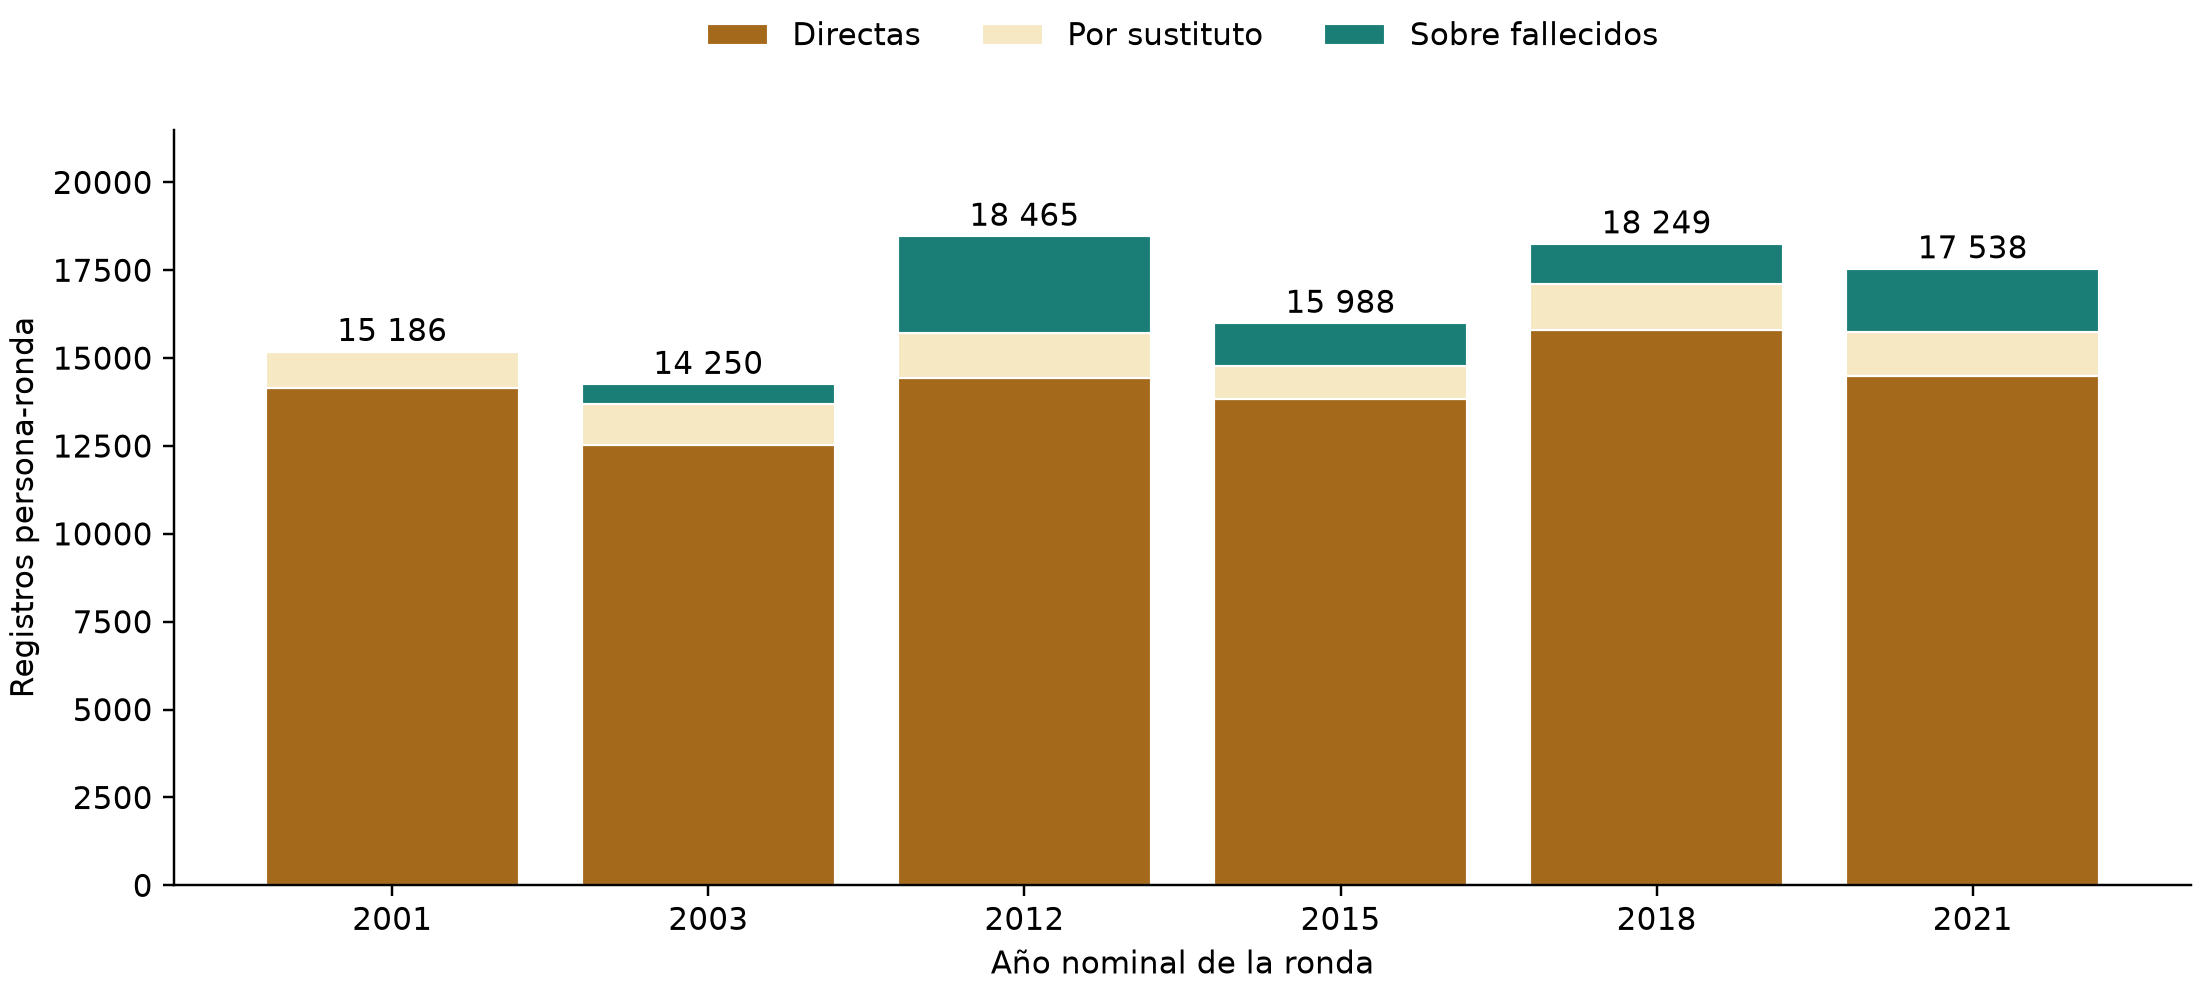
\includegraphics[width=\linewidth]{../resultados/figuras/figuras__borradores__cp1_modalidades.png}
 \caption[Registros por ronda y modalidad]{Registros por ronda y modalidad. Fuente: agregados de CP1, sin
 ponderación; todas las edades. Figura provisional para revisión editorial.}
 \label{fig:modalidades}
\end{figure}

\section{Incorporación, continuidad y ausencias temporales}

La primera aparición de una persona en el archivo se identifica mediante
$E_i=\min\{r:R_{ir}=1\}$. En una ronda, son incorporaciones observadas quienes
tienen $E_i=r$; son participantes previos quienes tienen $E_i<r$. Una
reaparición cumple simultáneamente presencia actual, presencia en alguna
ronda anterior y ausencia en la ronda inmediata precedente. Estas
definiciones dependen de la historia de registro, no de suponer equivalencia
con los códigos de muestra nueva del proveedor.

% Generado: no editar cifras manualmente.
\begin{table}[!htbp]
\centering
\caption{Incorporación y seguimiento por ronda}\label{tab:cp1-entradas}
\small\setlength{\tabcolsep}{4pt}
\renewcommand{\arraystretch}{1.15}
\begin{tabular}{lrrrr}
\toprule
\textbf{Año} & \textbf{N} & \shortstack[c]{\textbf{Primera}\\\textbf{presencia}} & \shortstack[c]{\textbf{Presencia}\\\textbf{previa}} & \textbf{Reaparición} \\
\midrule
2001 & 15\,186 & \shortstack[r]{15\,186\\(100,00\%)} & \shortstack[r]{0\\(0,00\%)} & \shortstack[r]{0\\(0,00\%)} \\
2003 & 14\,250 & \shortstack[r]{277\\(1,94\%)} & \shortstack[r]{13\,973\\(98,06\%)} & \shortstack[r]{0\\(0,00\%)} \\
2012 & 18\,465 & \shortstack[r]{5\,912\\(32,02\%)} & \shortstack[r]{12\,553\\(67,98\%)} & \shortstack[r]{357\\(1,93\%)} \\
2015 & 15\,988 & \shortstack[r]{650\\(4,07\%)} & \shortstack[r]{15\,338\\(95,93\%)} & \shortstack[r]{624\\(3,90\%)} \\
2018 & 18\,249 & \shortstack[r]{4\,823\\(26,43\%)} & \shortstack[r]{13\,426\\(73,57\%)} & \shortstack[r]{383\\(2,10\%)} \\
2021 & 17\,538 & \shortstack[r]{323\\(1,84\%)} & \shortstack[r]{17\,215\\(98,16\%)} & \shortstack[r]{1\,100\\(6,27\%)} \\
\bottomrule
\end{tabular}
\par\medskip
\parbox{\linewidth}{\footnotesize Fuente: elaboración propia con agregados de CP1, ENASEMsimple v2 (2001--2021). Frecuencias sin ponderación. Porcentajes sobre N de la ronda. Primera presencia + presencia previa = N. Reaparición es un subconjunto de presencia previa; primera presencia en el archivo no equivale automáticamente a modalidad de muestra nueva.}
\end{table}


La tabla~\ref{tab:cp1-entradas} permite reconciliar primeras apariciones y
participación previa con cada total. En 2012 hay \cpEntradasTres{} primeras
presencias y en 2018 \cpEntradasCinco{}, lo que contribuye al cambio de
composición respecto a las rondas anteriores. Las reapariciones suman
\cpReaparicionesTres{} en 2012, \cpReaparicionesCuatro{} en 2015,
\cpReaparicionesCinco{} en 2018 y \cpReaparicionesSeis{} en 2021. Son un
subconjunto de quienes ya habían participado, de modo que no deben sumarse
otra vez al total ni clasificarse como incorporaciones nuevas.

Para rondas consecutivas, la retención descriptiva se calcula como
\begin{equation}
 \widehat\rho_{r,r+1}=
 \frac{\sum_i R_{ir}R_{i,r+1}}{\sum_i R_{ir}}.
 \label{eq:retencion}
\end{equation}
El numerador incluye cualquier registro en destino. En consecuencia,
$\widehat\rho$ mide continuidad de presencia y no supervivencia. Las
entrevistas sobre fallecidos permanecen en el universo; un cambio de
modalidad no se confunde con ausencia.

% Generado: no editar cifras manualmente.
\begin{table}[!htbp]
\centering
\caption{Continuidad entre rondas nominales consecutivas}\label{tab:cp1-transiciones}
\small\setlength{\tabcolsep}{4pt}
\renewcommand{\arraystretch}{1.15}
\begin{tabular}{lrrrrr}
\toprule
\textbf{Transición} & \textbf{Años} & \textbf{N origen} & \textbf{Continúan} & \textbf{Retención (\%)} & \textbf{Ausentes} \\
\midrule
2001--2003 & 2 & 15\,186 & 13\,973 & 92,01 & 1\,213 \\
2003--2012 & 9 & 14\,250 & 12\,196 & 85,59 & 2\,054 \\
2012--2015 & 3 & 18\,465 & 14\,714 & 79,69 & 3\,751 \\
2015--2018 & 3 & 15\,988 & 13\,043 & 81,58 & 2\,945 \\
2018--2021 & 3 & 18\,249 & 16\,115 & 88,31 & 2\,134 \\
\bottomrule
\end{tabular}
\par\medskip
\parbox{\linewidth}{\footnotesize Fuente: elaboración propia con agregados de CP1, ENASEMsimple v2 (2001--2021). Frecuencias sin ponderación. Continúan + ausentes = N origen. La retención usa cualquier modalidad en destino, incluidas entrevistas sobre fallecidos. Los intervalos no son iguales y los porcentajes no son tasas anuales.}
\end{table}

% Generado: no editar cifras manualmente.
\begin{table}[!htbp]
\centering
\caption{Descomposición de las ausencias y retornos posteriores}\label{tab:cp1-ausencias}
\small\setlength{\tabcolsep}{4pt}
\renewcommand{\arraystretch}{1.15}
\begin{tabular}{lrrrr}
\toprule
\textbf{Transición} & \shortstack[c]{\textbf{Con}\\\textbf{fallecimiento}} & \shortstack[c]{\textbf{Sin}\\\textbf{fallecimiento}} & \shortstack[c]{\textbf{Retorno}\\\textbf{posterior}} & \shortstack[c]{\textbf{Sin retorno}\\\textbf{registrado}} \\
\midrule
2001--2003 & 0 & 1\,213 & 402 & 811 \\
2003--2012 & 546 & 1\,508 & 603 & 1\,451 \\
2012--2015 & 2\,741 & 1\,010 & 393 & 3\,358 \\
2015--2018 & 1\,209 & 1\,736 & 1\,066 & 1\,879 \\
2018--2021 & 1\,135 & 999 & 0 & 2\,134 \\
\bottomrule
\end{tabular}
\par\medskip
\parbox{\linewidth}{\footnotesize Fuente: elaboración propia con agregados de CP1, ENASEMsimple v2 (2001--2021). Frecuencias sin ponderación. Las dos primeras columnas de conteos dividen las ausencias según tipent=5 en la ronda inmediatamente anterior. Las dos últimas dividen esas mismas ausencias según retorno posterior observado; no sumar las cuatro. Sin retorno registrado no significa pérdida definitiva; 2021 es el cierre del archivo.}
\end{table}


La tabla~\ref{tab:cp1-transiciones} muestra variación en continuidad, con
intervalos nominales diferentes. La tabla~\ref{tab:cp1-ausencias} separa
ausencias tras una entrevista sobre fallecido en la ronda inmediatamente
anterior y ausencias sin ese antecedente. Esta segunda categoría no tiene
causa identificada por la comparación. También se examina retrospectivamente
qué ausencias son seguidas por una presencia posterior: ello demuestra
ausencia temporal de registro, pero no su causa ni supervivencia. La ausencia
sin retorno documentado hasta 2021 tampoco se denomina pérdida definitiva,
pues el archivo tiene un límite de observación.

Estas distinciones son esenciales para formular pares prospectivos. El
fallecimiento podría impedir observar un resultado económico de la misma
naturaleza; la sustitución podría cambiar la medición disponible; la ausencia
podría generar un resultado no observado. No se asignará la misma etiqueta a
estos procesos sin definir previamente el estimando. El tratamiento de muerte,
sustitución y ausencia permanece pendiente de revisión metodológica.

\section{Patrones de observación y atrición}

% Generado: no editar cifras manualmente.
\begin{table}[!htbp]
\centering
\caption{Número de rondas observadas por persona}\label{tab:cp1-participacion}
\small\setlength{\tabcolsep}{4pt}
\renewcommand{\arraystretch}{1.15}
\begin{tabular}{lrr}
\toprule
\shortstack[c]{\textbf{Rondas}\\\textbf{observadas}} & \textbf{Personas} & \textbf{Porcentaje} \\
\midrule
1 & 2\,025 & 7,45 \\
2 & 6\,635 & 24,42 \\
3 & 4\,445 & 16,36 \\
4 & 5\,589 & 20,57 \\
5 & 2\,172 & 7,99 \\
6 & 6\,305 & 23,20 \\
\bottomrule
\end{tabular}
\par\medskip
\parbox{\linewidth}{\footnotesize Fuente: elaboración propia con agregados de CP1, ENASEMsimple v2 (2001--2021). Frecuencias sin ponderación. Denominador: 27,171 personas únicas de 2001--2021. Presencia incluye cualquier modalidad; no equivale a entrevista directa.}
\end{table}


La distribución de $K_i$ en la tabla~\ref{tab:cp1-participacion} muestra que
\cpBalancePersonas{} personas aparecen en las seis rondas, equivalentes a
\cpBalancePorcentaje{} del universo de personas. La presencia en menos
rondas puede reflejar entrada tardía, fallecimiento, ausencia temporal o
cierre del seguimiento. El número de rondas no es, por sí mismo, una medida
de incumplimiento o abandono. La matriz individual de presencia se conserva
solo para cálculo interno; el notebook presenta intersecciones y patrones
agregados, sin identificadores.

\begin{figure}[tbp]
 \centering
 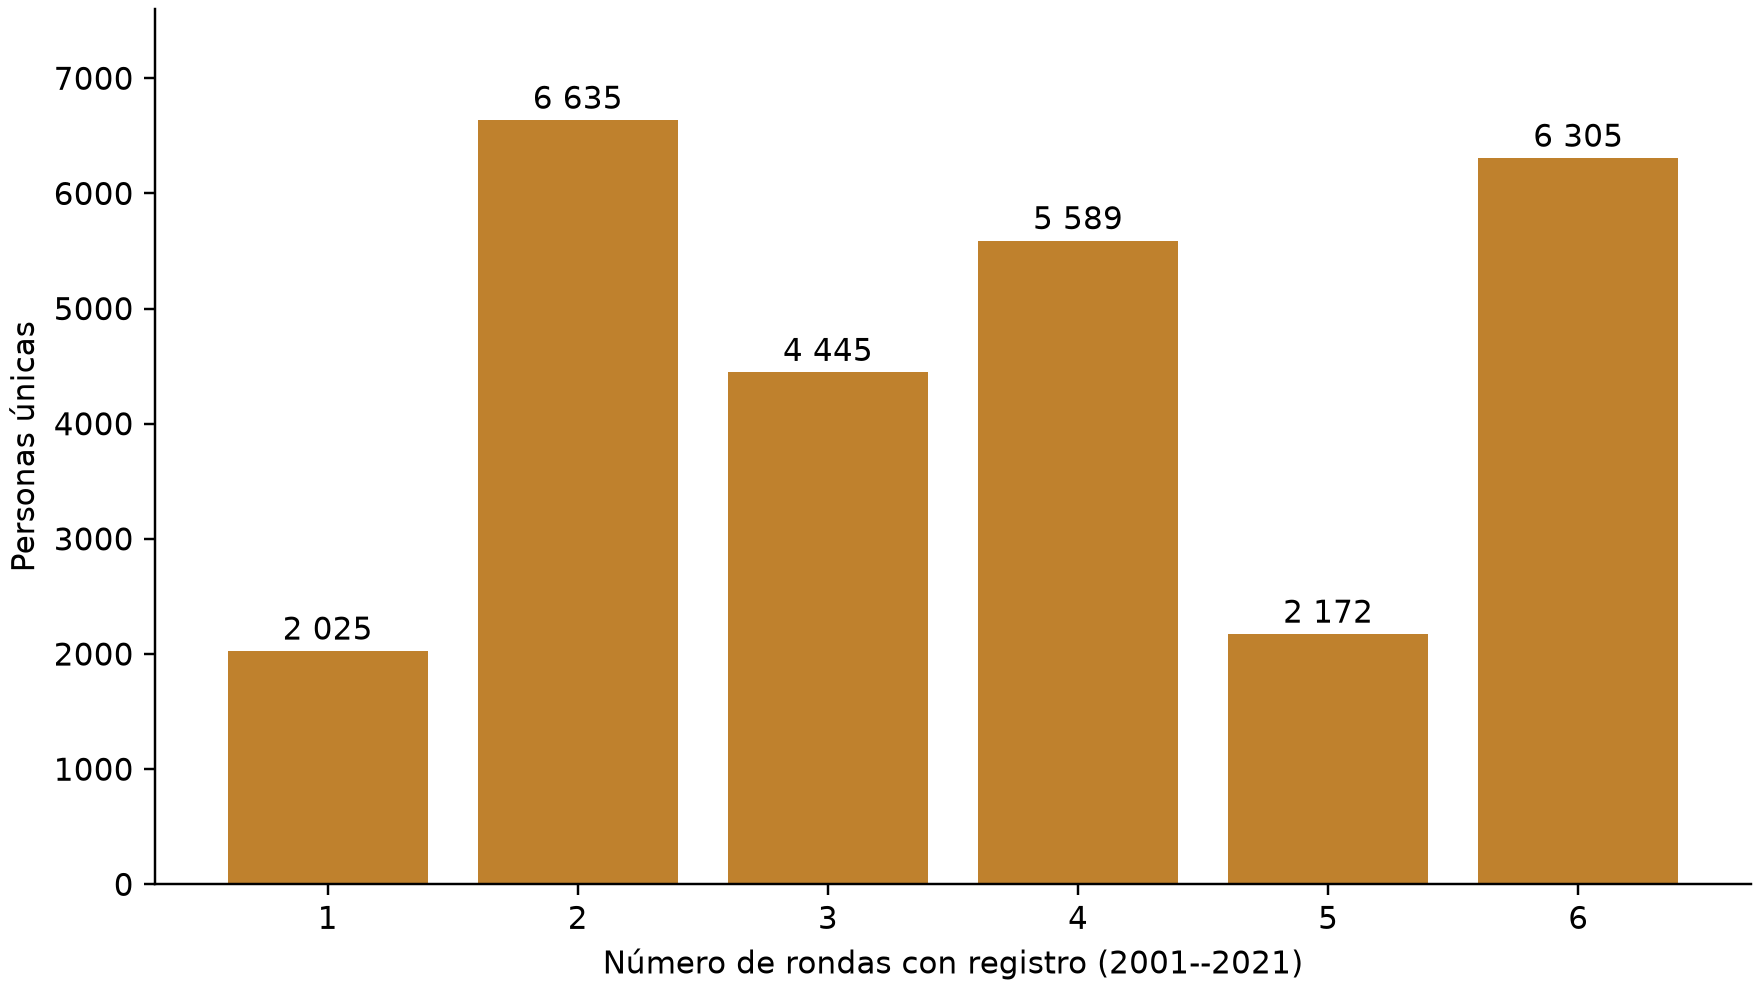
\includegraphics[width=0.90\linewidth]{../resultados/figuras/figuras__borradores__cp1_participacion.png}
 \caption[Personas según número de rondas con registro]{Personas según número de rondas con registro. Denominador:
 \cpTotalPersonas{} personas únicas; cualquier modalidad. Fuente: CP1, sin
 ponderación. Figura provisional para revisión editorial.}
 \label{fig:participacion}
\end{figure}

La continuidad completa selecciona una trayectoria futura y excluye entradas
tardías aun cuando tengan mediciones utilizables. Por esta razón no se
interpreta el panel completo como representativo por defecto. Las comparaciones
descriptivas de edad entre observados y ausentes en la ronda siguiente también
dependen de quién dispone de edad válida; los fallecidos permanecen en los
denominadores y a menudo no tienen esa variable. Estos contrastes sugieren
examinar selección, pero no estiman un efecto de la edad sobre abandono ni
cuantifican todavía sesgo en un modelo predictivo. El ajuste por atrición será
una evaluación posterior con supuestos explícitos.

\section{Valores faltantes, cobertura y ponderación}

La carga de Stata preserva los valores faltantes especiales antes de generar
una vista numérica para estadísticos. Se distinguen \variable{.f}
(reportado fallecido), \variable{.p} (información no incluida por sustituto),
\variable{.w} (no formulada en esa ronda), y las restantes causas de falta de
respuesta o invalidez del diccionario \citep{enasem2025simple}. Su reducción
prematura a un único faltante impediría distinguir indisponibilidad
estructural de falta de respuesta. No se convierten en cero ni se imputan
como parte de CP1.

% Generado: no editar cifras manualmente.
\begin{table}[!htbp]
\centering
\caption{Cobertura numérica de variables seleccionadas}\label{tab:cp1-cobertura}
\small\setlength{\tabcolsep}{4pt}
\renewcommand{\arraystretch}{1.15}
\begin{tabular}{p{0.20\linewidth}rrrrrr}
\toprule
\textbf{Variable} & \textbf{2001} & \textbf{2003} & \textbf{2012} & \textbf{2015} & \textbf{2018} & \textbf{2021} \\
\midrule
edad & \shortstack[r]{15\,186\\(100,00\%)} & \shortstack[r]{13\,693\\(96,09\%)} & \shortstack[r]{15\,701\\(85,03\%)} & \shortstack[r]{14\,775\\(92,41\%)} & \shortstack[r]{17\,094\\(93,67\%)} & \shortstack[r]{15\,729\\(89,69\%)} \\
sexo & \shortstack[r]{15\,186\\(100,00\%)} & \shortstack[r]{14\,250\\(100,00\%)} & \shortstack[r]{18\,465\\(100,00\%)} & \shortstack[r]{15\,988\\(100,00\%)} & \shortstack[r]{18\,249\\(100,00\%)} & \shortstack[r]{17\,538\\(100,00\%)} \\
educacion & \shortstack[r]{15\,167\\(99,87\%)} & \shortstack[r]{14\,151\\(99,31\%)} & \shortstack[r]{18\,371\\(99,49\%)} & \shortstack[r]{15\,808\\(98,87\%)} & \shortstack[r]{18\,089\\(99,12\%)} & \shortstack[r]{17\,214\\(98,15\%)} \\
est\_conyugal & \shortstack[r]{14\,730\\(97,00\%)} & \shortstack[r]{13\,703\\(96,16\%)} & \shortstack[r]{15\,723\\(85,15\%)} & \shortstack[r]{14\,779\\(92,44\%)} & \shortstack[r]{17\,114\\(93,78\%)} & \shortstack[r]{15\,739\\(89,74\%)} \\
urbano & \shortstack[r]{15\,186\\(100,00\%)} & \shortstack[r]{13\,704\\(96,17\%)} & \shortstack[r]{15\,723\\(85,15\%)} & \shortstack[r]{14\,779\\(92,44\%)} & \shortstack[r]{17\,114\\(93,78\%)} & \shortstack[r]{15\,739\\(89,74\%)} \\
a\_o\_ent & \shortstack[r]{15\,186\\(100,00\%)} & \shortstack[r]{14\,250\\(100,00\%)} & \shortstack[r]{15\,721\\(85,14\%)} & \shortstack[r]{14\,779\\(92,44\%)} & \shortstack[r]{17\,114\\(93,78\%)} & \shortstack[r]{15\,739\\(89,74\%)} \\
imp\_neto & \shortstack[r]{15\,127\\(99,61\%)} & \shortstack[r]{13\,671\\(95,94\%)} & \shortstack[r]{15\,723\\(85,15\%)} & \shortstack[r]{14\,745\\(92,23\%)} & \shortstack[r]{17\,094\\(93,67\%)} & \shortstack[r]{15\,716\\(89,61\%)} \\
orientacion & \shortstack[r]{0\\(0,00\%)} & \shortstack[r]{12\,495\\(87,68\%)} & \shortstack[r]{14\,448\\(78,25\%)} & \shortstack[r]{13\,850\\(86,63\%)} & \shortstack[r]{15\,786\\(86,50\%)} & \shortstack[r]{14\,484\\(82,59\%)} \\
serial7 & \shortstack[r]{0\\(0,00\%)} & \shortstack[r]{0\\(0,00\%)} & \shortstack[r]{0\\(0,00\%)} & \shortstack[r]{13\,850\\(86,63\%)} & \shortstack[r]{15\,786\\(86,50\%)} & \shortstack[r]{14\,484\\(82,59\%)} \\
\bottomrule
\end{tabular}
\par\medskip
\parbox{\linewidth}{\footnotesize Fuente: elaboración propia con agregados de CP1, ENASEMsimple v2 (2001--2021). Frecuencias sin ponderación. Cada celda: n válido y (\% sobre el total de la ronda). Se refiere a cobertura empírica, no a universo elegible ni respuesta entre vivos. El resto conserva sus motivos de faltante en los notebooks; cero valores válidos no equivale a ausencia del atributo.}
\end{table}


La tabla~\ref{tab:cp1-cobertura} presenta un subconjunto informativo de las
119 columnas auditadas. La cobertura varía por ronda y modalidad; tener una
columna no significa que su pregunta haya sido administrada a toda la muestra.
En particular, los ceros de cobertura de pruebas cognitivas en rondas sin
medición no indican ausencia de dificultad cognitiva. El inventario exhaustivo
de cada código y variable permanece en las seis fichas del notebook. Para
estadísticos continuos se utiliza el número de valores válidos, mientras que
las distribuciones categóricas conservan los faltantes dentro del total.

Los factores individuales \variable{factori_XX} y de hogar
\variable{factorh_XX} se auditan separadamente. Existen ceros y valores
positivos incluso en modalidades sobre fallecidos; la disponibilidad numérica
de un factor no acredita su pertinencia para un estimando dado. Todas las
tablas de este capítulo son frecuencias sin ponderación. No se suman factores
para llamarlos personas observadas, ni se trasladan factores transversales al
seguimiento como si fueran pesos longitudinales. El alcance de inferencia
poblacional exige una decisión adicional sobre universo, diseño y atrición.

\section{Auditoría de edad, sexo y fallecimiento}

% Generado: no editar cifras manualmente.
\begin{table}[!htbp]
\centering
\caption{Alertas de consistencia y denominadores}\label{tab:cp1-anomalias}
\small\setlength{\tabcolsep}{4pt}
\renewcommand{\arraystretch}{1.15}
\begin{tabular}{p{0.72\linewidth}r}
\toprule
\textbf{Control} & \textbf{n} \\
\midrule
Registros posteriores a primer fallecimiento & 3 \\
Personas con registros posteriores & 1 \\
Personas con códigos de sexo distintos & 1 \\
Pares adyacentes observados & 72\,505 \\
Pares con ambas edades válidas & 65\,031 \\
Pares con edad decreciente & 226 \\
Personas con edad decreciente & 225 \\
Pares que pasan de 60+ a menos de 60 & 48 \\
\bottomrule
\end{tabular}
\par\medskip
\parbox{\linewidth}{\footnotesize Fuente: elaboración propia con agregados de CP1, ENASEMsimple v2 (2001--2021). Frecuencias sin ponderación. Conteos agregados sin historias individuales. No se corrigen ni eliminan observaciones; una alerta no identifica cuál valor es correcto.}
\end{table}


La tabla~\ref{tab:cp1-anomalias} resume alertas sin corregir registros. Para
fallecimiento se identifica la primera ronda con \variable{tipent}=5 de cada
persona y se cuentan observaciones de rondas estrictamente posteriores.
Se detectan \cpMuerteRegistros{} registros posteriores de
\cpMuertePersonas{} persona: \cpMuerteDirectas{} directos y
\cpMuerteRepetidas{} nuevamente sobre fallecido.
Esta misma persona aporta la alerta de fallecimiento repetido. No son tres
personas ni duplicados de clave. La coincidencia de los dos indicadores
contemporáneos de fallecimiento no resuelve la contradicción longitudinal.
Son hipótesis posibles una clasificación de seguimiento incorrecta, una
revisión no propagada o un problema de enlace; falta contrastar el maestro,
las modalidades originales y la documentación de muerte. No se infiere una
fecha de muerte a partir de un año efectivo faltante.

Para sexo se cuenta el número de códigos válidos distintos dentro de una
persona. La alerta afecta a \cpSexoPersonas{} persona con \cpSexoRegistros{} registros
directos y códigos distintos; una moda no resuelve el empate. El proveedor
documenta que revisó sexo en la versión 2 mediante validación de discrepancias
de las variables originales \variable{sex_xx}
\citep[pp.~6--7]{enasem2025simple}. Se necesita verificar versión, variables
originales y enlace antes de decidir qué valor debe prevalecer. La alerta
no permite atribuir una causa individual.

Para edad se ordenan las observaciones por persona y ronda. Sea $r_i^{-}$
la ronda del registro observado inmediatamente anterior: se identifica un
descenso cuando
\begin{equation}
 D_{ir}=\mathbf{1}\{e_{ir}<e_{i,r_i^{-}}\},
 \quad \text{si ambas edades son numéricas válidas}.
 \label{eq:descenso-edad}
\end{equation}
Una ronda sin registro puede saltarse; una edad ausente en un registro
presente interrumpe la comparación y no se reemplaza por una edad válida
más antigua. De \cpParesObservados{} pares observados,
\cpEdadEvaluables{} son evaluables y \cpEdadNoEvaluables{} no.
Se reproducen \cpEdadPares{} descensos (\cpEdadPorcentaje{} de los pares
evaluables) en \cpEdadPersonas{} personas. Hay \cpEdadConsecutivos{} pares
entre rondas consecutivas y \cpEdadHuecos{} separados por una ronda ausente.
En \cpEdadCruce{} pares se pasa de edad registrada de 60 o más a menos de
60, con posible impacto en la elegibilidad por visita.

Todos los pares decrecientes presentan años efectivos crecientes y años de
nacimiento válidos sin cambios. Un contraste auxiliar comprueba si la edad
está en $[a_{ir}-b_{ir}-1,\ a_{ir}-b_{ir}]$, donde $b_{ir}$ es el año de
nacimiento declarado. En \cpEdadAnteriorIncompatible{} pares la edad anterior es incompatible y la
actual compatible, en \cpEdadActualIncompatible{} sucede lo contrario y en
\cpEdadAmbasIncompatibles{} ambas son incompatibles.
El intervalo es aproximado y depende de la veracidad de los años; no decide
qué edad es correcta ni certifica nacimiento. Un cumpleaños no explica por
sí solo un descenso cuando el año de entrevista avanza y el nacimiento
permanece estable. La magnitud, el modo de entrevista y los agregados
complementarios están documentados en el informe de revisión y el notebook.

La edad creada debe cotejarse con respuestas originales, fechas y reglas de
derivación. No se fuerza monotonicidad, no se reconstruye automáticamente
edad con nacimiento y no se eliminan casos. La ausencia de descenso tampoco
valida aumentos implausibles. Todas las alertas requieren un protocolo de
verificación antes de traducirse en reglas de inclusión o etiquetas.

\section{Comparación de alternativas de muestra}

% Generado: no editar cifras manualmente.
\begin{table}[!htbp]
\centering
\caption{Alternativas de muestra en todo el periodo}\label{tab:cp1-muestras}
\small\setlength{\tabcolsep}{4pt}
\renewcommand{\arraystretch}{1.15}
\begin{tabular}{p{0.24\linewidth}rrrrr}
\toprule
\textbf{Alternativa} & \textbf{Registros} & \textbf{Personas} & \textbf{\% personas} & \shortstack[c]{\textbf{Reg.}\\\textbf{excluidos}} & \shortstack[c]{\textbf{Pers.}\\\textbf{excluidas}} \\
\midrule
Universo completo & 99\,676 & 27\,171 & 100,00 & 0 & 0 \\
No balanceado & 99\,676 & 27\,171 & 100,00 & 0 & 0 \\
60+ por visita & 56\,004 & 18\,754 & 69,02 & 43\,672 & 8\,417 \\
Directas & 85\,248 & 26\,572 & 97,80 & 14\,428 & 599 \\
Directas 60+ & 50\,841 & 18\,158 & 66,83 & 48\,835 & 9\,013 \\
Seis presencias & 37\,830 & 6\,305 & 23,20 & 61\,846 & 20\,866 \\
Seis directas & 23\,358 & 3\,893 & 14,33 & 76\,318 & 23\,278 \\
Seis directas 60+ & 5\,784 & 964 & 3,55 & 93\,892 & 26\,207 \\
\bottomrule
\end{tabular}
\par\medskip
\parbox{\linewidth}{\footnotesize Fuente: elaboración propia con agregados de CP1, ENASEMsimple v2 (2001--2021). Frecuencias sin ponderación. Denominadores: 99,676 registros y 27,171 personas únicas. Personas conservadas: unión de claves con al menos una observación elegible. Cada filtro se compara independientemente con el universo; no hay una muestra predictiva aprobada.}
\end{table}


La tabla~\ref{tab:cp1-muestras} compara filtros independientes con el universo
original. El panel no balanceado permite de una a seis presencias y coincide
aquí con todo el universo; no significa excluir a quienes tienen seis rondas.
El filtro de 60+ por visita conserva \cpMayoresRegistros{} registros de
\cpMayoresPersonas{} personas, mientras que el filtro de directas conserva
\cpDirectasRegistros{} y \cpDirectasPersonas{}, respectivamente. La
intersección directa 60+ conserva \cpDirectasMayoresRegistros{} registros de
\cpDirectasMayoresPersonas{} personas. Estas personas únicas son la unión de
quienes mantienen al menos una observación elegible, no la suma de los
conteos anuales.

Exigir seis presencias conserva \cpBalanceRegistros{} registros de
\cpBalancePersonas{} personas; exigir seis directas reduce a
\cpBalanceDirectasRegistros{} y \cpBalanceDirectasPersonas{}; exigir además
60+ en cada visita reduce a \cpBalanceDirectasMayoresRegistros{} y
\cpBalanceDirectasMayoresPersonas{}. Los filtros cambian simultáneamente
continuidad, modalidad y composición por edad. No son definiciones
intercambiables y no se aprueba aquí ninguna muestra predictiva principal.
El apéndice~\ref{ap:tablas-cp1} muestra conservados y excluidos por ronda,
reconciliados con cada total original.

Otros criterios, como ser 60+ en la primera observación o permitir ingreso
desde la primera edad elegible, siguen comparados en el notebook. Su elección
dependerá de qué población y tiempo de entrada se pretenda representar.
Una alerta prospectiva no puede seleccionar observaciones por información
futura sin reconocer y justificar esa selección.

\section{Limitaciones y decisiones pendientes}

La unicidad de claves hace auditable el enlace, pero no garantiza veracidad
de todos los atributos. La cobertura heterogénea restringe qué predictores
pueden compararse entre rondas; las entrevistas por sustituto y sobre
fallecidos no proporcionan mediciones equivalentes a las directas. Las
primeras apariciones describen el archivo y no prueban todas las razones
institucionales de incorporación. La ausencia sin causa registrada y el
cierre en 2021 impiden clasificar pérdidas definitivas únicamente con los
patrones de presencia. Las frecuencias sin ponderación no se interpretan
como estimaciones nacionales.

Para el diseño económico, \variable{imp_neto} es patrimonio de la persona
y su cónyuge cuando corresponde, no un flujo de ingreso. Su uso exige
verificar precios, unidades, imputaciones y comparabilidad entre rondas antes
de establecer un umbral. Una posición relativa baja es una candidata
operativa que no se equipara sin discusión a pobreza ni a la medida de
vulnerabilidad de \citet{ligon2003}. Quedan pendientes el estimando, criterio
de edad/entrada, modalidad admisible, tratamiento de muerte y no observación,
alcance de ponderación y reglas de anomalías.

La futura comparación de modelos seguirá el protocolo del proyecto: misma
muestra de evaluación, mismos horizontes y particiones, transformaciones
aprendidas solo en entrenamiento e incertidumbre que respete dependencia
por persona. Se documenta aquí como requisito, no como validación ya ejecutada.
El cierre metodológico de CP1 sigue pendiente de revisión. La autora autorizó
iniciar el EDA independiente por bloques el 12 de octubre de 2026; esta autorización
no aprueba el estimando ni la integración definitiva. La escritura acompaña los resultados disponibles
sin convertir propuestas en decisiones definitivas.

% BEGIN CONSOLIDATED 03_pensiones_metodo
\section{Fuentes económicas y protocolo de clasificación pensionaria}
\label{sec:pensiones-metodo}

Los apartados siguientes conservan el protocolo documental anterior a la
integración. Su descripción de un enlace futuro debe leerse como antecedente
metodológico; la ejecución provisional y sus resultados se documentan en la
sección~\ref{sec:integracion-provisional}. El inventario nacional ampliado
se presenta en la sección~\ref{sec:catalogo-nacional}. Las condiciones de
validación no implican que se haya aprobado una homologación definitiva.


El complemento pensionario comienza con una auditoría de fuentes separadas,
antes de construir una base económica integrada. Se inspeccionaron completos
los 20 archivos Stata proporcionados: originales de K, archivos imputados,
secciones K individuales construidas, combinados de G/J/K/SA y ENASEMsimple.
También se revisaron las seis hojas del inventario Excel disponible. Las
fuentes contienen 5,368 columnas fuente-variable, incluidas las dos copias
individuales de 2018 y el archivo de 2024. El conteo describe cobertura del
inventario, no variables distintas ni observaciones independientes.

La lectura preservó las etiquetas y los valores faltantes especiales de Stata,
sin convertir categorías a textos. Para cada columna se registraron tipo,
etiqueta, conjunto de códigos etiquetados, número de filas y faltantes por
clase. Los códigos numéricos de negativa o desconocimiento permanecen sin
transformar: el número de valores no perdidos en Stata no equivale a un número
de respuestas sustantivas válidas. La determinación del universo elegible
requiere los saltos del instrumento. Esta etapa no calcula medias monetarias
que podrían incluir códigos numéricos especiales.

\begingroup\small\singlespacing
\setlength{\tabcolsep}{3pt}
\begin{longtable}{llrrp{4.4cm}}
\caption{Inventario de fuentes económicas revisadas}\label{tab:pensiones_fuentes}\\
\toprule \textbf{Fuente} & \textbf{Ronda} & \textbf{Registros} & \textbf{Variables} & \textbf{Clave única comprobada} \\
\midrule\endfirsthead
\toprule \textbf{Fuente} & \textbf{Ronda} & \textbf{Registros} & \textbf{Variables} & \textbf{Clave única comprobada} \\
\midrule\endhead\bottomrule\endfoot
F01 & 2012 & 10,427 & 164 & cunicah+subhog\_12 \\
F02 & 2015 & 9,921 & 212 & cunicah+subhog\_15 \\
F03 & 2021 & 10,716 & 180 & cunicah+subhog\_21 \\
F04 & 2018 & 17,094 & 125 & cunicah+np \\
F05 & 2018 & 17,094 & 125 & cunicah+np \\
F06 & 2024 & 14,076 & 507 & cunicah+subhog\_24 \\
F07 & 2012 & 10,427 & 648 & cunicah+subhog\_12 \\
F08 & 2015 & 9,953 & 756 & cunicah+subhog\_15 \\
F09 & 2018 & 11,401 & 543 & cunicah+subhog\_18 \\
F10 & 2021 & 10,716 & 524 & cunicah+subhog\_21 \\
F11 & 2003 & 8,895 & 348 & cunicah+acthog \\
F12 & 2001 & 9,811 & 328 & unhhid \\
F13 & 2001 & 15,186 & 62 & cunicah+codent01 \\
F14 & 2003 & 13,704 & 65 & cunicah+codent03 \\
F15 & 2012 & 15,723 & 66 & cunicah+np \\
F16 & 2015 & 14,779 & 156 & cunicah+np \\
F17 & 2021 & 15,739 & 129 & cunicah+np \\
F18 & 2003 & 8,895 & 165 & cunicah+acthog \\
F19 & 2001 & 9,811 & 146 & unhhid \\
F20 & 2001--2021 & 99,676 & 119 & cunicah+np+ronda \\
\end{longtable}
\noindent\footnotesize Fuentes F01--F20 se identifican por nombre completo en el inventario consolidado y su JSON. Ambas copias idénticas de 2018 se conservan. No sumar registros entre fuentes; existen universos solapados. El archivo 2024 queda separado.\par
\endgroup


El resumen de la tabla~\ref{tab:pensiones_fuentes} se acompaña de un diccionario
íntegro por archivo y una matriz variable--fuente, generados desde los metadatos.
La matriz contiene 1,917 candidatos léxicos tras retirar exclusivamente el sufijo
de ronda; esa operación facilita localizar columnas, pero no prueba equivalencia
conceptual. Todas las variables sustantivas quedan en el alcance del EDA futuro,
incluidos negocios, trabajo, activos, deuda, vivienda, donativos, gasto,
inseguridad alimentaria, apoyo familiar y los módulos de fallecimiento.
No se limita la revisión a ocho columnas finales.

\subsection{Unidad de observación y correspondencias comprobadas}

Los originales económicos y sus imputados tienen claves de entrevista de
hogar o subhogar; pueden contener flujos propios del informante, de su cónyuge
y conjuntos. Los archivos K individuales son productos construidos, no la
respuesta original de cada persona. La documentación del proveedor distingue
la construcción de ingresos individuales de la riqueza de hogar
\citep{enasemconstruidos,enasem2021imputacion}. Enlazar un hogar a dos personas
no autoriza adjudicar íntegramente un mismo monto a ambas.

Se comprobaron claves completas y únicas en todas las fuentes. Los individuales
de 2001 y 2003 usan, respectivamente, \variable{cunicah+codent01} y
\variable{cunicah+codent03}; los posteriores usan \variable{cunicah+np}.
Los originales de 2001 requieren un puente hacia \variable{unhhid}; los de
2003, un puente hacia \variable{cunicah+acthog} desde el individual construido.
El \variable{acthog} de ENASEMsimple no produce coincidencias directas con la
fuente económica de 2003. La coincidencia del nombre no garantiza la misma
codificación. Los ensayos de puente se limitaron a claves y validaron la
cardinalidad; no produjeron una base económica definitiva.

Todas las entrevistas directas de ENASEMsimple enlazan a los individuales
construidos en 2001, 2003, 2012, 2015 y 2021; en 2018 enlazan 15,766 de 15,786.
Los puentes a originales recuperan 14,099 de 14,154 directas en 2001 y 12,499
de 12,526 en 2003. En 2015 el original contiene 9,953 entrevistas económicas y
el imputado 9,921, y quedan 34 directas sin correspondencia en el imputado de
hogar. En 2021 hay 18 directas sin enlace al original/imputado de hogar,
aunque todas enlazan al individual. Estos resultados describen disponibilidad
y diferencias de universo, no ausencia de pensión o ingreso. La auditoría
completa conserva también los denominadores de todas las modalidades.

La huella SHA-256 acredita que las dos copias individuales de 2018 son
idénticas byte por byte. Ambas se inspeccionaron; no son dos muestras.
Las otras parejas de fuentes de la misma ronda se compararon por claves y
columnas comunes; el contraste de valores se restringió a claves únicas en
ambos lados. Las diferencias pueden reflejar imputación, derivación o versión,
y todavía no se atribuyen a una causa. El archivo imputado de hogar de 2018 y
los productos separados de ingreso total/patrimonio de 2018 y 2021 no se
identificaron entre los suministrados. Su existencia documental no acredita
su disponibilidad local.

\subsection{Definición de los ocho conceptos y estados de información}

Se mantienen las variables \variable{pension_contributiva},
\variable{pension_no_contributiva}, \variable{otro_apoyo_publico},
\variable{ayuda_familiar}, \variable{ingreso_pension_contributiva},
\variable{ingreso_pension_no_contributiva},
\variable{ingreso_transferencias_publicas} e \variable{ingreso_total}.
En esta entrega constituyen especificaciones de construcción: no se presentan
como variables armonizadas ya calculadas. La unidad objetivo es persona-ronda,
con titular, periodo, unidad monetaria y procedencia explícitos.

Los indicadores distinguirán recepción identificada, negativa explícita,
recepción de tipo desconocido, información faltante, pregunta no formulada
y no aplicabilidad. Solo una negativa con cobertura suficiente del concepto
permite codificar cero. Por ejemplo, desconocer el tipo de una pensión no
permite asignar simultáneamente cero a contributiva y no contributiva.
La recepción de una transferencia de una persona tampoco acredita parentesco.
Una prestación en especie se registra separadamente del flujo monetario.

\begin{table}[htbp]
\centering\small\singlespacing
\caption{Identificabilidad propuesta de los ocho conceptos económicos}\label{tab:pensiones_disponibilidad}
\begin{tabular}{p{5.1cm}cccccc}
\toprule \textbf{Concepto} & \textbf{2001} & \textbf{2003} & \textbf{2012} & \textbf{2015} & \textbf{2018} & \textbf{2021} \\
\midrule
pension contributiva & C & C & C & C & C & C \\
pension no contributiva & T & T & P & P & T & E \\
otro apoyo publico & P & P & P & P & C & C \\
ayuda familiar & T & T & C & C & C & C \\
ingreso pension contributiva & C & C & C & C & C & C \\
ingreso pension no contributiva & T & T & P & P & T & C \\
ingreso transferencias publicas & C & C & C & C & C & C \\
ingreso total & R & R & R & D & R & R \\
\bottomrule\end{tabular}
\par\medskip\begin{minipage}{\textwidth}\footnotesize
C: candidata condicionada; P: tipo parcial; T: agregado sin identificación suficiente; E: opción explícita de programa; D: total disponible del proveedor; R: reconstrucción o archivo adicional. No son resultados de recepción ni variables ya armonizadas.
\end{minipage}\end{table}


La tabla~\ref{tab:pensiones_disponibilidad} distingue la presencia física de
columnas de su identificabilidad. En 2001 se usan familias K55/K56/K58;
desde 2003 cambian a K58/K59/K61. En 2012 y 2015, las opciones de programas
federales o estatales permiten una clasificación parcial, sin nombre ni ámbito
inequívoco. En 2018, las fuentes de donativos públicos distinguen PROAGRO,
PROSPERA, INAPAM y otra institución, sin una opción explícita de pensión de
vejez. La opción de programas públicos en una pregunta de pensión futura no
prueba recepción actual \citep{inegi2018k}. En 2021 el cuestionario \citep{inegi2021k} incorpora una opción
explícita de Bienestar de personas adultas mayores en los apoyos propios y del
cónyuge. Esa mejora no elimina faltantes, ambigüedad de titular ni cambios del
periodo de referencia.

Los montos pensionarios agregados \variable{pens_t} o
\variable{inc_pension} no se tipifican automáticamente como contributivos.
Los totales \variable{tran_t} o \variable{inc_trans} tampoco equivalen sin
cotejo a transferencias exclusivamente públicas. Un mismo importe reportado,
derivado y luego imputado representa versiones de un componente; no se suman
como tres ingresos. Conservar las banderas de imputación permite evaluar la
sensibilidad en las mismas personas y periodos.

Para impedir doble conteo, el ingreso público incluye la prestación no
contributiva de vejez como un subconjunto. Una contabilidad propuesta es
\begin{equation}
 Y^{\mathrm{rec}}_{ir}=W_{ir}+B_{ir}+R_{ir}+C_{ir}
 +P^{\mathrm{con}}_{ir}+P^{\mathrm{sin\ tipo}}_{ir}
 +T^{\mathrm{pub}}_{ir}+T^{\mathrm{priv}}_{ir}+O_{ir},
 \label{eq:ingreso-componentes}
\end{equation}
donde trabajo, negocios, rentas, capital, pensiones y transferencias son
componentes mutuamente delimitados bajo una misma unidad y referencia.
$P^{\mathrm{no\ con}}$ no se vuelve a sumar porque está contenido en
$T^{\mathrm{pub}}$. La ecuación es una propuesta contable, no una definición
empírica aprobada: si falta un componente necesario, una suma parcial no se
presenta como ingreso total completo. \variable{income_15} existe en el
individual de 2015; los totales separados de 2018 y 2021 no están suministrados.
Los precios, periodicidades y fórmulas de los demás componentes deben cotejarse
antes de comparar cuantías entre rondas.

\subsection{Cronología, imputación y límites de integración}

La documentación de 2021 describe montos propios y de cónyuge, ingresos
individuales y riqueza de hogar, así como pasos adicionales que utilizan
información de 2018 para resolver ciertas atribuciones de 2021
\citep[pp.~6--8]{enasem2021imputacion}. Este antecedente obliga a conservar
procedencia y cronología del producto. No se supone que una imputación sea
una observación directa, ni que su disponibilidad retrospectiva garantice
que se hubiera conocido en el momento de una futura predicción. La ficha de
cada variable deberá registrar estas dependencias antes de usarla como señal
prospectiva.

La integración propuesta en el inventario conserva las 99,676 filas de ENASEMsimple mediante
uniones izquierdas validadas, sin sobrescribir edad, sexo, modalidad ni
cronología de CP1. Se exigirán relaciones uno-a-uno para fuentes individuales
y muchos-a-uno para hogar, indicadores de enlace y reconciliación de personas
y registros. Aún deben aprobarse titularidad, filtros, unidades, tratamiento
de fuentes no identificadas y equivalencias por pregunta. No se ha seleccionado
una muestra predictiva ni cambiado la definición económica pendiente.
La implementación provisional autorizada después de esa revisión se documenta
en la sección~\ref{sec:integracion-provisional}; no requiere cerrar primero
todos los bloques del EDA independiente.

El archivo de 2024 tiene 14,076 filas, 507 variables y clave única
\variable{cunicah+subhog_24}. Su fecha de versión en 2026 no es el año de ronda.
Se inventaría por separado: no existe una séptima ronda en el ENASEMsimple
proporcionado. Además, sus códigos de K79 distinguen vejez, discapacidad y ONG,
con numeración diferente de 2018 y 2021. Incorporarlo requeriría fuentes
individuales y puentes adicionales, revisión del instrumento y autorización
de la ampliación temporal. La referencia principal permanece en 2001--2021.
% END CONSOLIDATED 03_pensiones_metodo
% BEGIN CONSOLIDATED 03_eda_independiente_metodo
\section{Protocolo del análisis exploratorio independiente}
\label{sec:eda-independiente-metodo}

El análisis exploratorio se organiza en bloques de fuentes y rondas, conservando
la procedencia de cada medición. La autorización para iniciar esta etapa
descriptiva no establece una muestra predictiva, una definición de vulnerabilidad
ni una integración económica definitiva. La población registrada completa
continúa siendo la referencia; no se restringe inicialmente por edad, modalidad
de entrevista o continuidad de observación. Los resultados de integridad de CP1
conservan su alcance y sus decisiones pendientes.

La primera operación consiste en verificar que los archivos no hayan cambiado
respecto al inventario mediante sus sumas SHA-256, su estructura y sus conteos.
El control de cobertura incluye una fila por cada columna de cada fuente,
incluidas las copias idénticas y el archivo de 2024, que permanece fuera del
periodo principal. La prevalidación de códigos almacenados y faltantes se
distingue explícitamente del análisis sustantivo concluido. Los códigos de
negativa o desconocimiento se revisan por variable y cuestionario: no existe
una regla general que permita eliminar 8, 9, 88 o 99 en todas las mediciones.

En ENASEMsimple se elaboró un contrato por variable que identifica la página
del libro de códigos, la escala, la unidad, los códigos válidos y las
restricciones de interpretación \citep{enasem2025simple}. Los valores perdidos
especiales se contabilizan antes de la transformación numérica. La ausencia
de una pregunta, el salto por una respuesta previa, la entrevista por sustituto
y el fallecimiento se conservan como motivos distintos. Un valor fuera del
dominio documentado se registra separadamente; no se corrige ni se sustituye
automáticamente. Los valores extremos y los patrimonios negativos se mantienen.

Para una variable $v$ y ronda $t$, sea $N_t$ el número de registros y
$N^{\mathrm{val}}_{vt}$ el número con un valor disponible dentro del dominio
documentado. Para una categoría $c$, se presentan dos proporciones:
\begin{equation}
 p^{\mathrm{total}}_{vct}=\frac{n_{vct}}{N_t},
 \qquad
 p^{\mathrm{val}}_{vct}=\frac{n_{vct}}{N^{\mathrm{val}}_{vt}}.
 \label{eq:eda-denominadores}
\end{equation}
Ambas responden a preguntas distintas. La primera expresa la presencia de una
respuesta entre los registros de la ronda y la segunda describe la composición
de las respuestas válidas. Ninguna sustituye una proporción sobre el universo
elegible de la pregunta cuando este no se ha reconstruido. En particular, los
saltos laborales de \variable{autoem} y \variable{horas_trabajadas} requieren
cotejo adicional del instrumento; sus distribuciones se limitan a los valores
disponibles y no se presentan como prevalencias de toda la población.

La revisión posterior reconstruye el universo del indicador construido cuando
el libro documenta su disponibilidad por ronda y modalidad. Esta operación
conserva negativas, desconocimiento e interrupciones dentro del denominador
elegible; no utiliza el número de respuestas válidas como sustituto de dicho
universo. Si $N^{\mathrm{el}}_{vt}$ es el universo reconstruido y
$N^{\mathrm{val,el}}_{vt}$ las respuestas válidas en él, la cobertura es
$N^{\mathrm{val,el}}_{vt}/N^{\mathrm{el}}_{vt}$, definida solo si
$N^{\mathrm{el}}_{vt}>0$. Se auditan también valores válidos fuera del universo
propuesto. No disponibilidad instrumental implica universo cero y porcentaje
no definido; un filtro desconocido implica universo no determinado. Esta
distinción no reconstruye automáticamente todos los saltos de las preguntas
originales que alimentan el indicador.

Las medidas numéricas se describen mediante cuantiles, media, desviación
estándar, extremos y frecuencias de cero y valores negativos. Las categorías
nominales y ordinales se describen con frecuencias, sin interpretar la media
de sus códigos. Los histogramas emplean intervalos comunes entre rondas y
conservan las colas; el último intervalo incluye su extremo superior. Cada
lámina contiene seis paneles con la paleta BrBG y los denominadores explícitos.
Además se conserva una comparación conjunta por variable: porcentajes de todas
las categorías o P05, P25, mediana, P75 y P95 numéricos en una escala común,
junto con su tabla exacta. Los intervalos representan dispersión descriptiva,
no incertidumbre inferencial. Las ausencias no se grafican como tasas cero.
El desglose de modalidad distingue entrevistas directas de seguimiento y nuevas,
por sustituto de seguimiento y nuevas, y sobre fallecidos. Los porcentajes
son descriptivos sin ponderar y no constituyen estimaciones nacionales.

Las diferencias entre distribuciones de rondas describen composición, no
trayectorias individuales ni efectos causales. La escolaridad de primera
entrevista, las puntuaciones construidas y las banderas de imputación se
interpretan conforme a su procedencia. Antes de utilizar imputaciones del
proveedor como predictores será necesario verificar si su construcción empleó
información posterior al momento de la alerta. Esta etapa no demuestra ausencia
de fuga temporal ni estima desempeño predictivo. Tampoco compara crecimiento
patrimonial real mientras permanezcan pendientes las unidades, precios y
equivalencias entre fuentes económicas.

En el bloque independiente de K 2021, los montos derivados, imputados y las
banderas se cotejan dentro de cada archivo, sin unión definitiva entre fuentes.
Una recuperación corresponde a un derivado faltante con imputado disponible;
un cambio compara dos montos disponibles con tolerancia absoluta de 0.01 pesos
y relativa de $10^{-7}$. No se identifica de antemano la bandera con estas
operaciones: se verifica su concordancia empírica. Los ceros de productos
construidos pueden representar componentes no recibidos; su universo de
producto no es el universo de la pregunta monetaria entre receptores.
Los componentes del cónyuge requieren pareja: si el archivo carece del filtro,
el universo permanece no determinado. Cuando existe \variable{k52a_21},
el código 2 confirma pareja y el 1 excluye esa rama; una condición perdida
permanece desconocida. No se recupera el filtro de otra fuente mediante una
unión ni se deduce a partir de la disponibilidad del monto.

El cuestionario distingue la ventana retrospectiva de recepción de la
periodicidad solicitada para el monto. Negocios, rentas, pensiones ordinarias,
transferencias institucionales y consumo incluyen preguntas mensuales;
COVID y ventas/herencias solicitan montos totales. Los salarios permiten
periodo mensual o anual y su conversión no se da por validada sin verificar el
periodo del producto suministrado. Esta cautela responde a que el resumen
metodológico y el código del proveedor describen etapas distintas de
construcción \citep[pp.~4, 13--14 y apéndice]{enasem2021imputacion}.
En ningún caso se anualiza o deflacta automáticamente. La orientación de
ingresos propios o del cónyuge se audita solo mediante conteos internos de
punteros, sin publicar identificadores.
% END CONSOLIDATED 03_eda_independiente_metodo
% BEGIN CONSOLIDATED 03_integracion_provisional
\section{Integración longitudinal provisional de fuentes económicas}
\label{sec:integracion-provisional}

Tras revisar el inventario y los primeros análisis independientes, se autorizó
construir una base provisional sin esperar a terminar el EDA de todos los
archivos. Esta etapa resuelve la vinculación física y conserva la información
para nuevas verificaciones; no convierte la cobertura del enlace en validación
de titularidad, comparabilidad o elegibilidad de cada pregunta. La pregunta de
investigación y las decisiones predictivas pendientes permanecen vigentes.

\subsection{Identificación, cardinalidad y preservación del universo}

ENASEMsimple constituye el maestro de \intRegistros{} observaciones,
\intPersonas{} personas y seis rondas. Se conservan sus 119 variables, todas
las edades y modalidades, incluidos registros sobre fallecidos. La clave
personal es la concatenación estable de \variable{cunicah} y \variable{np}
con el separador ``:''; la observación queda identificada por
\variable{id+ronda}. Los componentes de texto conservan su formato y ceros
iniciales; los numéricos enteros se representan sin redondeo, relleno ni
notación científica. Se preservan también valores y formatos Stata del
maestro, sin reconstruir supuestos ceros iniciales de campos numéricos.
\variable{ano} representa la ronda nominal, mientras \variable{a_o_ent}
conserva el año efectivo de entrevista.

Para cada fuente económica $E_s$ se aplica una unión izquierda al maestro
$M$, validando la unicidad de la clave derecha antes del enlace:
\begin{equation}
M^{(s)}=M^{(s-1)}\;\mathop{\Join}\limits_{\mathrm{izquierda},\,k_s}\;E_s,
\qquad |M^{(s)}|=|M|.
\label{eq:integracion-izquierda}
\end{equation}
Las fuentes individuales requieren cardinalidad uno a uno dentro de ronda;
las fuentes de hogar admiten muchas personas hacia un único registro
económico. Claves incompletas no se emparejan entre sí y duplicados derechos
detienen el procedimiento. No se elige arbitrariamente una primera fila para
resolver conflictos ni se enlaza por \variable{cunicah} aisladamente.

En 2001, el individual construido enlaza mediante
\variable{cunicah+codent01} y aporta \variable{unhhid} para el hogar. En 2003,
\variable{cunicah+codent03} permite trasladar el \variable{acthog} económico;
el homónimo del maestro no produce una correspondencia directa válida. En
2012, 2015, 2018 y 2021 se emplean \variable{cunicah} y el subhogar específico
de cada ronda. Los puentes preservan el \variable{np} original del maestro.
Estos pasos se verifican individualmente en el notebook de integración.

\subsection{Procedencia, faltantes y titularidad}

Se incorporan \intFuentes{} fuentes económicas distintas, manteniendo
\intColumnasFuente{} columnas fuente, incluida la maestra. Cada campo
económico lleva el prefijo de su fuente y metadatos de producto original,
imputado o construido. La copia binaria idéntica del individual 2018 se
representa una vez con el alias documentado; 2024 sigue fuera del periodo.
Los indicadores de imputación y códigos originales desconocidos o no
aplicables se conservan, sin sumarlos como componentes adicionales.

Parquet almacena valores y etiquetas de faltantes Stata por separado. Un
auxiliar identifica el tag original cuando existe; el estado de enlace
distingue ausencia de fuente en la ronda, clave incompleta, falta de puente y
no correspondencia. Así, un null por unión no pierde su diferencia frente a
\variable{.f}, \variable{.p}, \variable{.w}, negativa o desconocimiento
numérico. Las cadenas vacías también se mantienen. Se comprueba la igualdad
de todas las columnas, filas y tags al releer el archivo, no solo su dimensión.

Un hogar puede aportar contexto económico a varias personas sin que sus
ingresos pertenezcan a todas ellas. La atribución personal se inicia en 2021,
cuyo instrumento y producto construido fueron cotejados
\citep{inegi2021k,enasem2021imputacion}. Se exige orientación
\variable{key_21}, coincidencia del NP del titular en hogar e individual y
rama de pareja válida. El puntero K45d por sí solo no enumera el bloque K58;
para pensiones se exige también la orientación del proveedor. Los registros
sobre fallecidos se conservan, pero no acreditan recepción personal actual.
Una discrepancia impide derivar el indicador y conserva los originales para
revisión.

Las preguntas afirmativas de pensión permiten conservar múltiples slots,
instituciones, año de inicio y montos observados mensuales; se mantienen los
casos de institución o monto desconocido. IMSS e ISSSTE identificados aportan
evidencia de sistema contributivo, incluyendo derechos derivados; no prueban
cotización personal ni régimen específico. Instituciones agrupadas,
privadas, extranjeras o personas permanecen sin tipo validado. La opción 5
de K79/K82 identifica el apoyo de vejez; otros programas públicos se
distinguen e INAPAM no se interpreta automáticamente como pensión monetaria.
El instrumento combina dinero y especie, limitación que se conserva.

El número derivado es un mínimo de declaraciones/slots con evidencia; una
suma observada es parcial y no ingreso total. No se añaden versiones
imputadas a los montos reportados ni se completa un faltante con cero.
Las demás rondas mantienen todas las columnas disponibles y una homologación
pendiente de titular, filtros, periodicidad y selección múltiple. Estas
variables auxiliares no cierran las ocho especificaciones previamente
acordadas ni resuelven el deflactor, ponderación o diseño prospectivo.
% END CONSOLIDATED 03_integracion_provisional
% BEGIN CONSOLIDATED 03_titularidad_pensiones
\section{Auditoría específica de titularidad pensionaria}
\label{sec:titularidad-metodo}

La vinculación de una entrevista económica de hogar con registros individuales
no determina por sí misma quién recibe una prestación. Esta auditoría distingue
la pensión del beneficiario de la fila, la recepción de su pareja residente y
la presencia de ingresos pensionarios declarados en la entrevista económica.
La unidad individual conserva la clave \texttt{id+ronda}, mientras que el
agregado económico utiliza la clave del hogar o subhogar de cada levantamiento.
El producto integrado anterior permanece intacto; se genera un conjunto de
auxiliares privados separado y versionado, sin eliminar variables fuente.

En las rondas tempranas, el proveedor describe una orientación de los ingresos
propios y de la pareja basada en controles de entrevista y códigos del informante.
En 2001 intervienen J1 y los controles de orden de entrevista; en 2003 se utiliza
K96a y el código personal histórico; en 2012 y 2015 se coteja K96a con NP
\citep{enasem2001imputacion,enasem2003imputacion,enasem2012imputacion,enasem2015imputacion}.
Los campos \texttt{key} de los productos individuales se verifican contra sus
componentes pensionarios construidos: una orientación relativa de la fila no
debe confundirse con los códigos absolutos de persona denominados CLAVE en
los documentos históricos. La concordancia numérica acredita el funcionamiento
de esa orientación, pero no sustituye los controles originales ausentes.
En particular, 2001 conserva una clasificación candidata del proveedor, con
comprobación independiente pendiente. Para informantes externos de 2003--2015
no se reproduce la asignación basada en orden de entrevista sin sus controles.

En 2018 y 2021, los punteros \texttt{k45d} y \texttt{k52a\_1} identifican por NP
a los titulares de las dos ramas económicas \citep{enasem2018imputacion,enasem2021imputacion}.
Se exige concordancia del puntero seleccionado entre el producto individual
y el original de hogar; en 2021 se coteja además \texttt{key\_21}. Si el NP del
sujeto corresponde a la rama de cónyuge, esa rama constituye su pensión propia,
aunque su pareja haya sido informante. Una rama no puede identificar a dos
personas distintas. La recepción de la pareja requiere cotejar también el otro
puntero y la rama de pareja; la concordancia del titular propio no resuelve
automáticamente el otro beneficiario. Los punteros discordantes, la orientación ausente y los
registros sobre fallecidos no acreditan recepción personal actual.

Los libros de códigos originales requieren un tratamiento monetario por ronda:
en 2001/2003 los montos pensionarios codifican negativa y desconocimiento como
888888 y 999999, mientras que desde 2012 utilizan 8888888 y 9999999
\citep{enasem2001codigosk,enasem2003codigosk}. Estos valores permanecen en la
fuente y se excluyen únicamente del monto analítico correspondiente.

El indicador de recepción K toma valor positivo ante una afirmativa en
jubilación, viudez, invalidez o accidente de trabajo, u otras pensiones; toma
valor negativo solo ante cuatro negativas explícitas. Las respuestas de
negativa a contestar, desconocimiento y los faltantes preservan su estado.
El filtro de ausencia de pareja residente se aplica solo cuando está
documentado en el archivo, sin deducirlo de respuestas ausentes. La recepción
del programa de vejez de 2021 se mantiene separada: K79/K82 admite dinero o
especie y una negativa del bloque K58/K64 no demuestra ausencia de toda
protección previsional \citep{inegi2021k}.

El doble conteo se controla mediante un registro lógico de prestaciones.
Sea $\mathcal{E}_{ht}$ el conjunto de slots originales únicos de un hogar
$h$ en la ronda $t$, distinguidos por rama beneficiaria y contingencia.
La suma observada parcial se define como
\begin{equation}
 M^{\mathrm{obs}}_{ht}=\sum_{e\in\mathcal{E}_{ht}:\,m_e\ \mathrm{observado}}m_e.
 \label{eq:titularidad-agregado}
\end{equation}
Este objeto descriptivo no es ingreso pensionario completo: excluye montos
desconocidos y no incorpora una segunda versión imputada del mismo slot.
Cuando no existe ningún monto observado, el agregado analítico es desconocido,
en lugar de cero. En el registro individual solo corresponden los eventos de
su beneficiario; la réplica de una pregunta de hogar en dos filas de personas
no genera dos prestaciones. En 2012/2015 las instituciones se seleccionan por
contingencia y no necesariamente identifican de forma unívoca cada slot.
Dos pensiones de igual institución e importe no se eliminan si corresponden a
beneficiarios o slots distintos.

La viudez se asigna a quien recibe efectivamente la prestación, no a la persona
fallecida que generó el derecho. Las preguntas sobre heredar en el futuro una
pensión no acreditan cobro. Los montos antes y después del fallecimiento
K101/K103 y las transferencias mixtas por divorcio, separación o supervivencia
se conservan como fuentes separadas y pendientes de reconciliación; no se
añaden automáticamente al bloque pensionario principal. Esta auditoría no
cierra las ocho especificaciones de armonización ni aprueba ponderación,
deflactor o muestra predictiva.
% END CONSOLIDATED 03_titularidad_pensiones
% BEGIN CONSOLIDATED 03_proteccion_economica
\section{Armonización descriptiva de pensiones y apoyos gubernamentales}
\label{sec:proteccion-metodo}

La protección económica se estudia mediante fuentes de recepción que complementan
el patrimonio y permiten describir su distribución entre perfiles demográficos.
Se reutilizan la base integrada provisional y la auditoría de titularidad de la
sección~\ref{sec:titularidad-metodo}; no se repiten las uniones ni se modifica el
maestro. La muestra descriptiva corresponde a edad de 60 años o más en cada visita,
sin exigir continuidad ni entrevista directa. Esta selección no aprueba la muestra
predictiva. Los registros sobre fallecidos no acreditan cobro contemporáneo y
permanecen en el universo longitudinal para estudiar seguimiento. La edad faltante
no permite establecer elegibilidad por edad y se contabiliza por separado.

Se definen dos indicadores documentales distintos. $P_{it}^{K}$ indica recepción
propia en las cuatro contingencias de K: jubilación, viudez, incapacidad y otra.
$A_{it}$ identifica donativos públicos adicionales en dinero o especie durante
el año previo a la entrevista. El bloque K no corresponde exclusivamente a
prestaciones contributivas y el bloque A no corresponde exclusivamente a
pensiones no contributivas. La pregunta sobre apoyos excluye el ingreso ya
mencionado; esta regla del instrumento no acredita que toda respuesta esté libre
de duplicación. No se construye un ingreso total sumando K y A.

En 2001 se utiliza K76a para el informante económico y K79a para su cónyuge;
en 2003 y desde 2012 se emplean K79a y K82c. Las ramas se orientan al beneficiario
auditado, que puede ocupar el apartado del cónyuge si respondió su pareja.
La orientación propia y el puntero de la otra persona se evalúan separadamente.
La respuesta 1 acredita recepción y 2 acredita negativa; NR, NS, faltantes y
enlaces no comprobados conservan estado desconocido. Ni un monto positivo ni
una imputación sustituyen la pregunta de recepción. Las reglas tempranas y sus
límites están documentados en \citet{enasem2001codigosk,enasem2003codigosk,
enasem2012imputacion,enasem2015imputacion}.

Hasta 2015 los donativos no identifican el programa individual: los ejemplos de
la pregunta no constituyen respuestas sobre programa. En 2018 se registran hasta
dos instituciones y en 2021 se agrega explícitamente el programa de vejez junto
con modificaciones de nombres \citep{inegi2018k,inegi2021k}.
Se conserva cada versión temporal. La opción 5 en 2021 identifica el programa de
vejez en este bloque, mientras INAPAM y una institución no especificada no se
convierten en una pensión monetaria. IMSS/ISSSTE acreditan la familia de seguridad
social, incluidas prestaciones derivadas; los demás organismos y regímenes
requieren evidencia adicional. Las categorías federales/estatales agrupadas de K
no permiten asignar nombre, ámbito ni monto individual por programa.

Los cruces distinguen recepción, coexistencia, apoyo con negativa K, apoyo con
pensión desconocida y negativas suficientes de los dos bloques. La última categoría
se denomina ``negativas K y A'', sin afirmar ausencia de toda prestación o ayuda
privada. Para un perfil $g$, se calculan por separado la proporción mínima observada
sobre el universo elegible y la tasa entre respuestas conocidas:
\begin{equation}
 \widehat r_{g,t}^{\mathrm{conocida}}=
 \frac{n_{g,t}^{\mathrm{si}}}{n_{g,t}^{\mathrm{si}}+n_{g,t}^{\mathrm{no}}},
 \qquad
 \widehat r_{g,t}^{\mathrm{elegible}}=
 \frac{n_{g,t}^{\mathrm{si}}}{N_{g,t}^{\mathrm{elegible}}}.
 \label{eq:proteccion-tasas}
\end{equation}
N elegible incluye personas vivas de 60+ en la visita; N conocido depende de
la recepción y de su cobertura documental. La composición de receptores emplea
otro denominador, $n_{g,t}^{\mathrm{si}}/\sum_g n_{g,t}^{\mathrm{si}}$.
Ninguna de estas cantidades resuelve la selección por no respuesta.

Los controles proceden de ENASEMsimple: sexo 1/2, edad de visita, educación en años
a partir de primera entrevista y localidad según un corte de 100 mil habitantes
\citep{enasem2025simple}. Este último indicador no identifica ruralidad estricta:
las localidades menores de 100 mil incluyen asentamientos urbanos. Se evita
etiquetarlo como rural. Los grupos de escolaridad son 0, 1--5, 6, 7--9 y 10 o más
años; describen años aprobados, sin certificar títulos escolares. Se mantienen
los desconocidos en todas las tablas y las anomalías de CP1 sin corrección.

Las asociaciones categóricas se describen dentro de ronda mediante
\begin{equation}
 V=\sqrt{\frac{\chi^2}{n\min(r-1,c-1)}}.
 \label{eq:proteccion-asociacion}
\end{equation}
Se informa $n$ de pares conocidos y la presencia de celdas esperadas pequeñas.
Spearman complementa los contrastes ordinales de edad
y escolaridad. Los análisis trivariados estratifican K--A por sexo/localidad,
K--educación por sexo y K--edad por localidad. No se apilan rondas como personas
independientes ni se informan pruebas poblacionales sin diseño validado.
Los ponderadores transversales disponibles no se aplican automáticamente a esta
selección ni a transiciones longitudinales; los resultados describen la muestra.

Los eventos monetarios permanecen separados por fuente, versión, beneficiario,
contingencia y posición. Se agregan una vez por evento de hogar, aun cuando el
enlace lo replique en dos personas; la medición individual selecciona exclusivamente
su beneficiario. No se suman montos propios y del cónyuge para denominar ingreso
personal, ni originales e imputados como componentes adicionales. Los montos
observados describen un mes normal nominal; no prueban frecuencia normativa de
entrega ni permiten inferir cambios de poder adquisitivo. En 2015 se documenta
la discrepancia de códigos monetarios entre cuestionario y libro, sin alterar
los valores originales ni efectuar correcciones automáticas.

Las transiciones emplean la cohorte viva de 60+ en origen y todos los registros
maestros para clasificar la observación final. Se distingue muerte registrada,
ausencia con reaparición posterior, ausencia sin retorno observado, edad final no
elegible y recepción desconocida. Inicio, continuidad y pérdida son cambios
observados solo en pares de comparabilidad conceptual condicionada, no fechas
administrativas ni impactos causales. Se señalan rupturas K en 2003/2012 y
2015/2018, y A en 2018/2021. J1/orden 2001, los punteros discordantes y las
33 coincidencias de 2015 siguen pendientes; no se aprueba la clasificación final.
% END CONSOLIDATED 03_proteccion_economica

% BEGIN CONSOLIDATED 03_recuperacion_metodologica
\section{Conciliación con el diseño longitudinal del borrador original}
\label{sec:recuperacion-metodologica}

El documento original desarrolla una distinción necesaria entre observación
persona-ronda y unidad analítica de transición. Una persona puede aportar
varios pares de observaciones; estos pares conservan dependencia dentro de
su historia y no se consideran realizaciones independientes por defecto.
La información previa permite examinar cambios acumulados, mientras una
sola pareja de visitas permite estudiar solamente el intervalo que delimita.
Esta ventaja de la historia extensa no requiere excluir, para toda la
investigación, a quienes ingresaron tarde o tuvieron ausencias temporales.

El borrador proponía seis entrevistas directas para el análisis principal.
El diseño vigente conserva el universo de CP1 y el panel abierto. Ambas
propuestas responden a poblaciones diferentes: la primera condiciona a
continuidad y capacidad de entrevista directa hasta una fecha futura,
mientras la segunda permite examinar continuidad, mortalidad y reemplazo
del informante. El panel completo se mantiene como alternativa de
sensibilidad y no como estimando aprobado. Las restricciones de aplicación
de pruebas cognitivas deben justificarse por medición; no se aplican a
todas las variables económicas únicamente porque compartan una fila.

La información sobre factores de expansión se conserva. Sin embargo,
seleccionar el factor individual de cada ronda solo crea una columna de
peso transversal disponible; no valida un ponderador longitudinal para
el subconjunto de sobrevivientes o para los pares predictivos. Los resultados
descriptivos de protección económica permanecen sin ponderar. La inferencia
nacional requerirá comprobar universo, estratos, unidades primarias,
modalidades cubiertas y ajuste apropiado al estimando. La disponibilidad de
un peso no sustituye esos requisitos.

\subsection{Resultado patrimonial: propuesta de notación sin decisión de umbral}

El PDF alterna primer cuartil, primer quintil y los subíndices 25 y 20.
Esta inconsistencia se registra para revisión, en lugar de corregirla mediante
una elección sustantiva automática. Una representación general que permite
discutir ambas alternativas es
\begin{equation}
 V_{it}^{(\alpha)}=\mathbf{1}\{W_{it}\leq q_{\alpha,t}(\mathcal P_t)\},\qquad
 E_{i,t\to s}^{(\alpha)}=
 \mathbf{1}\{V_{it}^{(\alpha)}=0,\;V_{is}^{(\alpha)}=1\},
 \label{eq:umbral-pendiente}
\end{equation}
donde $W$ representa la medida patrimonial, $\mathcal P_t$ la población de
referencia y $\alpha$ el nivel del cuantil. El primer cuartil corresponde a
$\alpha=0{,}25$ y el primer quintil a $\alpha=0{,}20$. Esta ecuación es una
propuesta conceptual: no se calculan aquí cortes, eventos ni prevalencias
de vulnerabilidad. La elección de $\alpha$, la población, ponderación,
empates y sensibilidad deben aprobarse conjuntamente. Si varias
observaciones comparten el corte, la proporción clasificada puede exceder
el porcentaje nominal del cuantil.

Un corte reestimado en cada ronda mide posición relativa dentro de una
distribución cambiante. Para una futura evaluación prospectiva habrá que
definir además cuándo está disponible el umbral de destino y cómo se evita
utilizar el conjunto de prueba en el ajuste de transformaciones. Los
predictivos futuros solo podrán emplear cambios calculados hasta $t$:
$\Delta X_{it}=X_{it}-X_{i,t^-}$ requiere una visita anterior realmente
observada y mediciones comparables. Las señales de deterioro propuestas en
el original no se validan por asignarles umbrales de dos puntos o dos
síntomas; su escala, disponibilidad y fundamento siguen pendientes.

La dimensión laboral también requiere interpretación. La salida del empleo
puede corresponder a retiro previsto, incapacidad, desempleo u otras
circunstancias; no se codifica automáticamente como deterioro económico.
La localidad se describe mediante el corte de cien mil habitantes de
\variable{urbano}, no como ruralidad estricta. La escolaridad corresponde
a los años declarados en la primera entrevista y la edad a la visita;
esas referencias temporales impiden tratar los perfiles como exposiciones
idénticas y actualizadas en cada ocasión \citep{enasem2025simple}.

La conciliación conserva el propósito de alerta temprana y las dimensiones
de salud física, salud mental, cognición, funcionalidad y participación.
Las hipótesis actuales continúan como propuestas de trabajo: el PDF
original no contiene H1--H3 terminadas. Las decisiones predictivas no se
derivan de los contrastes descriptivos ni de la recuperación editorial del
documento. La matriz de conciliación y el apéndice de pendientes separan
contenido recuperado, decisiones vigentes y cuestiones aún abiertas.
% END CONSOLIDATED 03_recuperacion_metodologica

% BEGIN CONSOLIDATED 03_exploracion_pensionaria
\section{Exploración pensionaria y estrategia abierta de investigación}
\label{sec:exploracion-metodo}

La autora autorizó una modificación explícita de estrategia el 12 de octubre de
2026. Esta etapa estudia la distribución y las trayectorias de las pensiones
para formular preguntas sustentadas en los datos; no adopta todavía pregunta
definitiva, hipótesis principal, variable objetivo, definición de vulnerabilidad
ni modelo. La alerta temprana se conserva como antecedente y posibilidad futura.
El universo de CP1 y los productos de integración y titularidad permanecen
inalterados. Esta ampliación reutiliza esos productos y evita repetir las
uniones o deducir titularidad a partir de la presencia de ingresos del hogar.

La selección exploratoria exige edad registrada de al menos 60 años en cada
visita, sin continuidad obligatoria ni restricción inicial a entrevistas
directas. Se reproduce una muestra de 56\,004 personas-ronda de 18\,754 personas;
el maestro conserva 99\,676 registros de 27\,171 personas. Un filtro central
configurable devuelve una copia y comprueba la unicidad de \texttt{id+ronda}.
La función existente concatena \texttt{cunicah:np}, con separador, sin sustituir
los códigos personales históricos ni modificar sus formatos almacenados.
Los registros sobre fallecidos se preservan en el maestro y el seguimiento;
no se interpretan como ingresos actuales de una persona viva. La edad
contemporánea ausente no se rellena para incluirlos en una muestra de 60+.

La organización conceptual distingue columnas, versiones y conceptos.
Las 8\,668 columnas se trazan individualmente, incluidas claves, indicadores de
faltantes y controles. La clasificación léxica de las columnas sin contrato
se presenta como candidata y requiere revisión documental. Los contratos
previos de ENASEMsimple y K2021 se vinculan al mapa, sin tratar nombres parecidos
como equivalencias verificadas. Original, imputado, construido y armonizado
conservan su procedencia; solo eventos originales previamente orientados
alimentan las nuevas distribuciones de recepción e institución.

Se distinguen recepción propia, del cónyuge, ambas, negativas de ambas ramas y
estado conjunto desconocido. Esta última categoría exige prudencia: una
respuesta propia afirmativa puede coexistir con desconocimiento del cónyuge,
por lo que el cuadro conjunto no sustituye la tasa propia. Una negativa K solo
corresponde a las contingencias capturadas en K. El donativo A no identifica
siempre programa, prestación no contributiva o entrega monetaria separada de
especie. Las instituciones múltiples cuentan personas por institución y nunca
replican el monto por cada selección. El número de slots observados se distingue
del número total declarado; todavía no existe un contrato equivalente validado
de este último para las seis ondas. Las prestaciones de viudez se adjudican al
beneficiario del evento, no a quien generó originalmente el derecho.

Para cada cruce se separan $N_{\mathrm{total}}$, elegibilidad potencial,
respuestas conocidas y desconocidas. La prevalencia de rama cónyuge en toda
la muestra no equivale a la tasa entre personas con pareja elegible. Los
No operativos ante ausencia explícita de rama cónyuge residente se conservan;
no son respuestas brutas negativas ni prueban ausencia de prestaciones de
una pareja no residente. La categoría conjunta de negativas contiene esos
No derivados. Solo en 2018/2021 se confirma aquí el universo de pareja mediante
filtro y punteros; el universo temprano permanece desconocido. Una tasa dentro
de un grupo $g$ es
\begin{equation}
 r_g=\frac{\sum_{i\in g}\mathbb{1}(K_i=\mathrm{sí})}
 {\sum_{i\in g}\mathbb{1}(K_i\in\{\mathrm{sí},\mathrm{no}\})},
 \qquad
 c_g=\frac{\sum_{i\in g}\mathbb{1}(K_i=\mathrm{sí})}
 {\sum_i\mathbb{1}(K_i=\mathrm{sí})}.
 \label{eq:exploracion-tasa-composicion}
\end{equation}
El primer cociente expresa recepción entre respuestas conocidas dentro del
grupo y el segundo, composición del conjunto receptor. Ambos denominadores
son distintos y excluyen incertidumbre de manera explícita. Los universos de
los indicadores construidos se recuperan de la revisión B01, sin equipararlos
al universo exacto de cada pregunta bruta. Para salario principal se exige
orientación personal y filtro afirmativo de trabajo asalariado; los demás
registros no reciben salario cero. Los montos salariales con mes/año pendientes
no se convierten ni se agregan como ingreso total.

La edad se divide en 60--64, 65--69, 70--74, 75--79 y 80 o más. La escolaridad
inicial se agrupa en 0, 1--5, 6, 7--9 y 10 o más años; no se atribuye adquisición
educativa entre visitas. \texttt{urbano} distingue menos de 100 mil frente a
100 mil o más habitantes, no ruralidad estricta. \texttt{ocupacion} representa
condición de actividad y combina retiro, incapacidad y ausencia de trabajo
\citep[pp.~17--18, 58--59]{enasem2025simple}. El patrimonio es un stock del
entrevistado y su pareja, mientras la pensión se orienta individualmente; se
conservan ceros, negativos y cuantiles descriptivos sin construir un outcome.

La V de Cramér describe asociación categórica entre respuestas conocidas y
Spearman, relaciones de rangos compatibles con las escalas. Se conservan los
N válidos, exclusiones y celdas esperadas pequeñas. No se realizan pruebas
confirmatorias, no se afirma significancia y no se seleccionan relaciones por
una dirección esperada. Al explorar numerosos contrastes, la búsqueda de
patrones no equivale a confirmación de hipótesis. Los ponderadores y el diseño
permanecen sin validar para estos estimandos: los resultados describen la
muestra, no tasas nacionales. Las distribuciones monetarias son nominales y
se interpretan dentro de onda, sin crecimiento real ni suficiencia aprobada.

En seguimiento se parte de personas vivas de 60+ en origen y se conservan sus
perfiles iniciales. A diferencia de las matrices J02, una edad menor a 60 o
faltante en destino no elimina retrospectivamente la persona: se conserva el
estado pensionario documentado salvo entrevista sobre fallecido. No se corrige
la edad. Fallecimiento, ausencia con retorno posterior, ausencia sin retorno
observado y recepción desconocida permanecen separados. Los intervalos
nominales son dos, nueve y tres años. Solo se interpreta inicio, continuidad o
pérdida observada cuando los contratos son condicionadamente comparables;
no se infiere un cambio administrativo ni el efecto de una política.
% END CONSOLIDATED 03_exploracion_pensionaria
